\section{Evaluation}

We evaluated Berth's cold-start performance against a non-predictive baseline that relies on a generic runtime and does not utilize warm pooling.

\subsection{Experimental Setup}
Benchmarks were conducted on a Linux host executing automated deployment requests for a mixed set of Node.js, Python, and Go repositories. Latency was measured from the moment the API received the \texttt{POST /environments} request until the container achieved a \texttt{RUNNING} state with all dependencies installed.

\subsection{Cold-Start Latency}
As detailed in Table \ref{tab:coldstart}, Berth drastically outperforms the baseline configuration. The integration of predictive pre-warming reduces the median (p50) initialization time by approximately 67\%, demonstrating the effectiveness of the static analysis heuristic. Figure \ref{fig:cdf} plots the cumulative distribution function (CDF) for the initialization times.

\begin{table}[t]
\caption{Cold-start latency comparison (20 sandboxes, 5 concurrent)}
\label{tab:coldstart}
\centering
\begin{tabular}{lccc}
\toprule
\textbf{Configuration} & \textbf{p50 (s)} & \textbf{p95 (s)} & \textbf{p99 (s)} \\
\midrule
Baseline (no prediction, no warm pool) & 30.3 & 57.7 & 65.7 \\
Berth (prediction + warm pool)         & 9.0  & 13.2 & 15.1 \\
\bottomrule
\end{tabular}
\end{table}


\begin{figure}[htbp]
\centerline{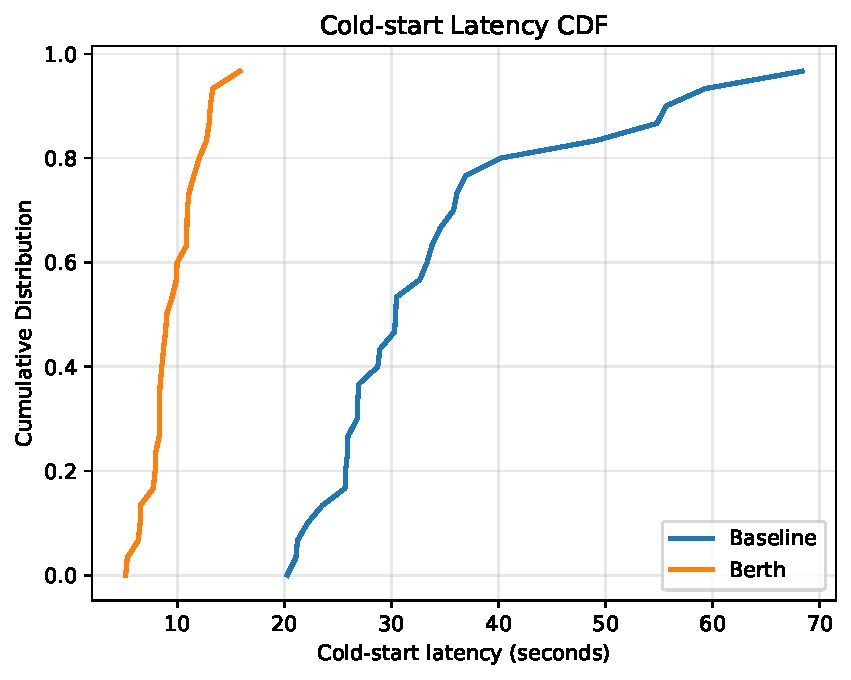
\includegraphics[width=\columnwidth]{figures/coldstart-cdf.pdf}}
\caption{Cumulative Distribution Function of cold-start latency comparing Baseline vs Berth.}
\label{fig:cdf}
\end{figure}
